\part{Basics of Numerical Computation}
\thispagestyle{plain}

How we write what algorithms is informed by how we represent data. While
there exist exotic approaches like analog computers that can e.g. handle
integration elegantly \citep{Ulmann2020} or quantum computing which
might e.g. at some point accelerate machine learning \citep{biamonte2017quantum},
standard binary data representation is vastly prevailing.

Binary data can be very efficiently and reliably stored and operated on (see figure \ref{fig:basics_computation}),
but the respective chosen representations might come with caveats.

\begin{figure}

    \centering

    \begin{subfigure}{0.4\textwidth}
      \centering
      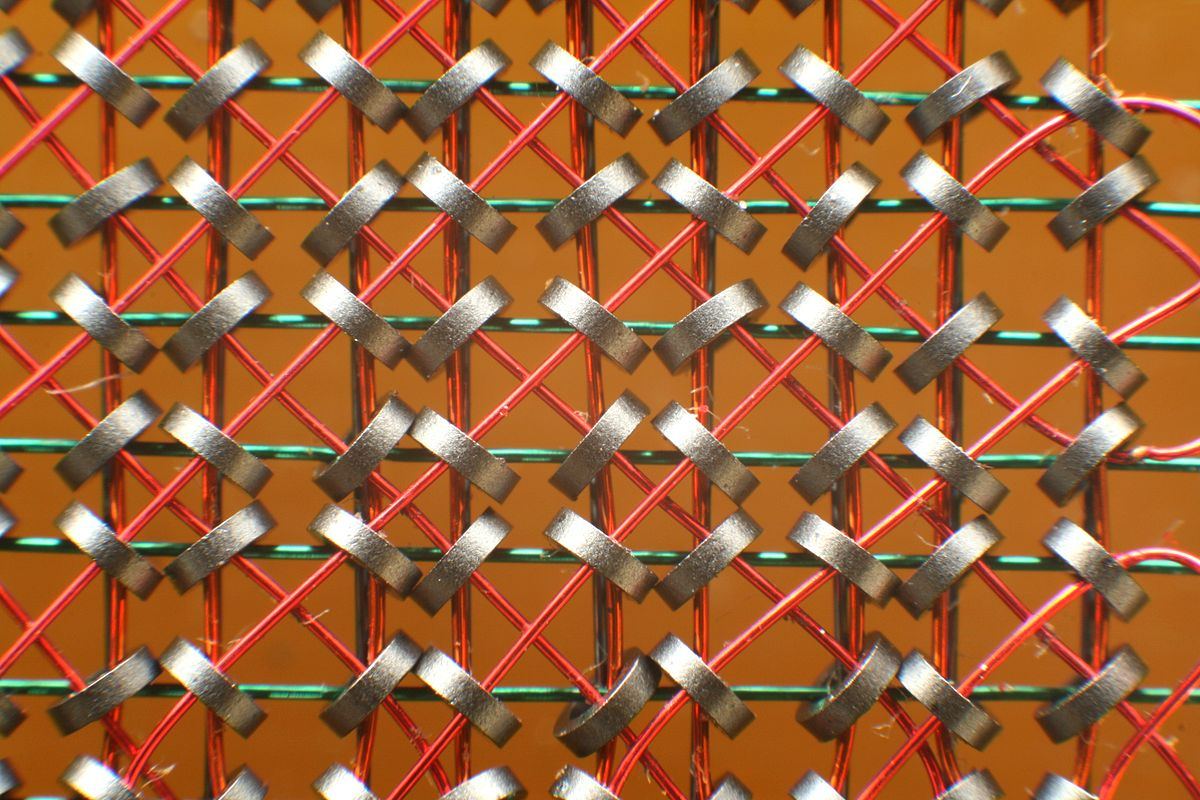
\includegraphics[width=.95\linewidth]{figures/magnetic_memory.jpg}
      \caption{Historic Magnetic Core Storage. Bits are stored as the direction of magnetic flux.}
      \label{fig:mcore}
    \end{subfigure}\hspace{0.1\textwidth}%
    \begin{subfigure}{0.4\textwidth}
      \centering
      \includesvg[width=.95\linewidth]{figures/mosfet.svg}
      \caption{Field-effect transistor (more specifically MOSFET schematic). Power-efficiently switching currents is at the heart of modern computing. Based on a Floating-Gate or Charge-Trapping mechanism and the tunnel effect, storage can be realized via stored charges.}
      \label{fig:fet}
    \end{subfigure}

    \begin{subfigure}{0.5\textwidth}
        \centering
        \includesvg[width=.95\linewidth]{figures/nand.svg}
        \caption{NAND-Gate. Bit operations lie at the core of computations.}
        \label{fig:nand}
    \end{subfigure}

    \caption{Basics of Computation.}
    \label{fig:basics_computation}

\end{figure}